\clearpage
\section{Theoretische Grundlagen}
\subsection{Doppelbrechung}
Es existieren Materialien in denen die Lichtgeschwindigkeit $v$ in alle Richtungen gleich ist und Materialien in welchen die Lichtgeschwindigkeit für verschiedene Richtungen verschiedene charakteristische Werte aufweist. Im ersten genannten Fall spricht man von einem optisch isotropen Medium, im zweiten von einem optische anisotropen Medium.\\
In einem optisch isotropen Medium gib es somit einen Brechungsindex n welcher durch den Quotienten aus $c$ und $v$. Bei optisch anisotropen Materialien geht diese skalare Größe in einen Tensor $n_{ij}$ mit $i,j = 1, ...,3$ über. Um nun die Ausbreitungsgeschwindigkeit einer linear polarisierten Welle zu beschreiben, führt man das Indexellipsoid ein, welches gegeben ist durch:
\[ \sum\limits_{i,j=1}^{3} B_{ij} x_j x_i = 1 ~~,~~ wobei ~ B_{ij}=\frac{1}{n_{ij}^2} .\]

\begin{floatingfigure}[l]{5.5cm}
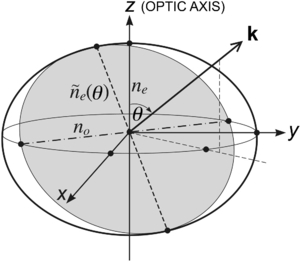
\includegraphics[scale=1.5]{ellipso}
\caption{Ellipsoid zum Bestimmen der charakteristischen Lichtgeschwindigkeit, Quelle: [iop]}
\label{fig:ellipso}
\end{floatingfigure}

Eine senkrecht zur Ausbreitungsrichtung der Lichtwelle stehende Ebene schneidet das Indexellipsoid auf einer Ellipse. Die Längen der Halbachsen geben die Größe des Brechungsindex an, für eine Lichtwelle welche in entlang der Halbachse linear polarisiert ist. Da wir jede Lichtwelle durch eine Superposition aus zwei entlang der Halbachsen polarisierten Wellen beschreiben können, erhalten wir zwei mit unterschiedlicher Geschwindigkeit ausbreitende Wellen. Dies nennt man Doppelbrechung.